\section{Briefly About USB}
\label{sec:usb_briefly}

Disclaimer: This chapter is heavily copied from the documentation of the
previous project \textit{USB subsystem in HelenOS}\cite{helenos:helusb} and filled in with the new
features and specifics of USB 3.

This chapter provides a brief overview of the USB architecture. It does not aim
to be a drop-in replacement for Universal Serial Bus specifications. It can be
also viewed as a summary of what the reader of this document must already know.
If you are new to USB, you can use this chapter as a starting point for further
reading.

\subsection{The ‘Big’ Picture}

USB is a technology used for connecting peripherals to host computer. Its main
advantages are simplicity of usage for end users, pretty good scalability (in
terms of number of simultaneously attached devices) and a choice of possible
transfer types that accommodate requests of diametrically different devices.
The USB defines the following aspects (most of them will be mentioned later in
this chapter):

\begin{itemize}
\item bus physical topology
\item physical interface — both mechanical (plugs) and electrical
\item power management
\item configuration of attached devices
\item querying attached devices for supported functions
\item low-level data protocol used on the bus
\item high-level data protocol — transfer types
\end{itemize}

The following sections will describe parts that are most important for
programmers of USB-related software, such as device drivers or host
controllers. They will not include description of low-level aspects, such as
electrical current settings or sizes of mechanical plugs. The acronym USB is
used in two slightly different meanings in the following text. First, as a
common prefix (e.g.\ USB device), second in its original meaning, describing the
bus itself (when the word ‘bus’ is used, it will always refer to the Universal
Serial Bus unless explicitly stated otherwise).

\subsection{Bus Topology}

USB uses a tree-like physical bus topology. In the root of the tree there is
the host computer with a hardware chip — host controller — controlling all
communication over the bus. All communication requests of device drivers are
directed to the driver of the host controller that schedules them and then
sends them to the USB ‘wire’. The host controller provides several
\textit{ports} to which devices are connected.

USB devices come in two flavors. First, there are \textit{functions} — these
provide actual functionality and create leaf nodes in the bus topology. An
example of an USB function is a printer or a keyboard. The other kind are
\textit{hubs} that create branches on the bus and to which the other devices
might be connected.

Hubs provide means to attach more devices to the same bus. The attachment place
is called a port (typical hubs for PCs has about four ports). Each hub has two
different kinds of ports. First, there is the upstream port through which the
hub is connected to a parent device (i.e. the predecessor in the tree) and then
there are several downstream ports through which the other devices are
connected. The host controller must always provide at least one port to allow
device attachment. Typically, the ports provided by the host controller are
provided by its own hub, called \textit{root hub}.

All USB versions must be backwards compatible in a sense that if you connect
the latest-version USB device to a most recent USB host controller through
USB 1.0 hub, the communication will use the protocol as specified by USB 1.0.
For the drivers, the precise protocol version used usually does not mean much,
differences are described in terms of different \emph{speeds}. Knowledge of the
speed the device operates on is important for proper scheduling.
%
\begin{itemize}
	\item \textbf{USB 1} defines \emph{low} and \emph{full} speeds (OHCI, UHCI, xHCI)
	\item \textbf{USB 2} defines \emph{high} speed (EHCI, xHCI)
	\item \textbf{USB 3} defines \emph{super} speed (xHCI only)
\end{itemize}

Looking at the list of controllers supporting individual speeds you can see
that EHCI is missing for low and full speeds. EHCI supports only high-speed
devices on its root hub ports. There must be either a companion controller
sharing physical plugs or an embedded high-speed hub to support low- and
full-speed devices too.

The correlation between speeds and USB protocol version resulted in unclear
distinction between them. Unless explicitly stated, a ``high-speed device''
refers to a device compatible with USB 2.0 that is able to communicate at high,
full, and low speeds. Counterintuitively, ``super-speed device'' is a device
that operates using the USB 3 protocol. This is due to the dual-bus topology
explained in section \ref{sec:dual-bus}.

Although physically, the topology is a tree rooted in the host controller,
the topology is abstracted by the HC. In USB~1, hubs are just transparent
splitters that add no logic to the bus. USB~2 adds high-speed hubs, which can
isolate environments of different speeds. USB 3 with its dual-bus topology is
even more complex -- every USB~3 hub behaves as two almost-separate hubs,
a regular high-speed one and another super-speed only. When a device is
connected, a decision is made on which one it will show up. Furthermore, USB~3
allows to control separate bus instances for arbitrary subsets of roothub
ports. Also, every link is now separate full-duplex link, so that hubs now must
be smarter and employ a Store and Forward paradigm. The difference is similar
to the difference between Ethernet hubs and switches -- a virtual bus topology
has changed to a routed star topology.

Each device connected to a bus instance receives a unique address (a
positive integer) and reacts only to communication that is targeted to it.
Before the device receives this address, it listens on the \textit{default
address} (number zero). To prevent situation when more devices would listen on
the default address simultaneously, each hub must provide means to disable
communication forwarding to certain ports (USB terminology says that hub does
not \textit{signal} on given downstream port). USB 3 with separated instances
uses a different mechanism, a \emph{Route String}, which contains the number of
downstream port on every tier to route the packet to its destination.

\subsection{Device Configurations, Interfaces and Endpoints}

USB was designed to be as flexible regarding device configurations as possible.
Because of this, each device can provide several \textit{configurations}. Each
configuration may provide completely different sets of features but in reality
practically almost all common USB devices have only a single configuration.

Each configuration can provide one or more \textit{interfaces}. The interface
provides the actual functionality of the device. For example, an USB printer
provides the printing as an interface. Some devices may provide multiple
interfaces. For example, a digital camera may provide an interface for direct
communication with the camera (usually via vendor-specific drivers) and, as a
fallback, a mass-storage interface that can be used to download photos when the
specialized drivers are not available.

Each interface can have several \textit{alternate settings} that change device
capabilities at the interface level. For example, network card may offer
several alternate settings using different sizes of data packets, or cameras
offering an alternate setting for each supported resolution.

The actual communication with the device performed through \textit{endpoints}.
Each endpoint belongs to a single interface and represents a communication
‘gate’ to the device — USB uses the term \textit{pipe} to describe an abstract
connection between the device driver on one side and the device on the other
one. Endpoints are usually unidirectional (exceptions are control endpoints)
and they have several attributes that must be obeyed by the driver.

A special endpoint — \textit{control endpoint zero} (also called default
control endpoint) — is present on each device and is used for configuration
purposes and for standard requests (e.g. for querying the device for
generic capabilities).

\subsection{Bus Protocol and Transfer Types}

The USB defines how data that are supposed to be sent to (or received from) a
device shall be encoded and treated prior to their sending over the wire. This
overview skips the physical aspect of the communication and starts with an
abstraction, that the host controller has, which is a way to send a stream of
bytes using the wire.

Communication over the bus uses data \textit{packets} which encapsulate the
actual payload and some service data. The service data include target address,
endpoint number, packet type and data needed for packet integrity checks.

Before moving on to describing packet types, it is necessary to mention
transfer types. In order to allow devices with different transfer requirements
(e.g. web camera that supplies a continuous stream of data vs. keyboard with
a few bytes several times a minute) the transfers (and therefore endpoints) are
divided into four different types.

The first type of transfers are \textit{control transfers}. These are used for
the device configuration and for manipulating the state of the device. Every
device has at least the default control endpoint but it is possible for the
device to have multiple control endpoints. The control transfers are
bidirectional.

The second type are \textit{interrupt transfers}. These are intended for small
and infrequent data where minimizing the latency is the primary goal. These are
considered periodic transfers and the host controller reserves a part of the
bus bandwidth for them. The typical devices using this transfer type are all
HID devices.

The third type of transfers are \textit{bulk transfers}. Bulk transfers are
used to send large chunks of data over the bus when the requirements are to
have correct data, but there are no strict requirements on latency. Typical
devices include printers, scanners or external disks. USB 3 also introduces
streams as an another layer of abstraction over bulk transfers.

The last type of transfers are \textit{isochronous transfers}. Unlike bulk
transfers, where data integrity is a priority, isochronous transfers ignore
data integrity and all priority is put on quick and periodic delivery (policy
is that delayed data are worse than damaged ones). Multimedia devices such as
web-cameras or wireless controllers use this transfer type.

When a device driver wants to send data to the device (the device cannot
initiate the transfer), it gives the payload to the host controller together
with information about target device (address) and endpoint. It must also
provide information about transfer type and data direction. For incoming
transfers, it instead reserves the data buffers to which the device can send
the data. The host controller then encapsulates these information and issues
USB packets on the bus. This is already part of the abstraction xHCI provides,
the xHCI driver only instructs the hardware to do so. Former HC interfaces had
to schedule the individual transfers into USB \emph{frames} (a time unit on
which USB is synchronized).

The protocol is roughly the same for bulk, interrupt and isochronous
transfers. Control transfers are a bit different because they have a special
preamble — a setup packet. The setup packet contains commands that might
change the device state and this packet might be optionally followed by a data
phase. The control transfers are the only ones that are actually bidirectional
(because the setup packet is always outgoing, while the data phase could be
either in or out).

\subsection{Device Descriptors and Device Classes}

In previous sections querying USB device for its capabilities was mentioned.
This section will describe this querying in more detail. Each USB device must
provide several data blocks, called \textit{descriptors}, describing its
configuration and capabilities. Some descriptors are device-dependent while
others are generic for any USB device.

The roughest description of a device is provided in a \textit{device
descriptor}. It holds information about device vendor, device class (see
below), number of possible configurations and several other details.

Each configuration is then described by a \textit{configuration descriptor}.
This descriptor also contains the number of interfaces the configuration
provides. Each interface is then described by an interface descriptor. The
interface descriptor specifies which class the interface belongs to and how
many endpoints it specifies.

Unsurprisingly, each endpoint is described by an \textit{endpoint descriptor}.
This descriptor defines attributes of the endpoint — data direction, transfer
type and endpoint number.

In case of USB 3, an endpoint descriptor is followed by a \textit{superspeed
endpoint companion descriptor}. This defines USB 3 specific features such as
bulk streams.

The descriptors can be viewed as a tree, where the device descriptor is the
root node that has several descendants — configurations. Each configuration
then groups interfaces and endpoint descriptors are leaves. Device may provide
its own descriptors (e.g. vendor-specific ones) that may stand aside of this
tree or be part of it (then they are typically inserted somewhere between
interfaces or endpoints).

Although logically the descriptors form a tree, the device usually returns them
in a serialized manner. For example, interface and endpoint descriptors can be
retrieved only as a part of a configuration descriptor they belong to. The
ordering in the serialized form implies the logical tree it represents.

USB was designed with flexibility of offered functionality in mind but to
prevent total chaos, devices (or rather their functionality) were divided by
common attributes into so called \textit{device classes}. Each class deals with
devices of certain kind, e.g. HID devices, printers, scanners, audio or a
special vendor class for any device that would not fit into any other one. Some
classes define \textit{subclasses} for fine-grained resolution (e.g. HID class
offers subclasses for keyboards and mice).

The class is reported as a part of device and interface descriptor. That is
because a single physical device may provide functionality of several classes
simultaneously, depending which interface the software communicates with. In
such cases the class reported through the device descriptor is a special value
with meaning ‘no class, see interface’.

\subsection{Bus Enumeration}

USB was designed with possibility of hot-plugging and thus it has to have
well-defined actions when a new device is added. The following is a simplified
sequence of what all the involved drivers and devices must go through. The
setup is that new device is attached to some hub that is already initialized
and configured.

\begin{enumerate}
\item The hub (the hardware) detects change on one of its ports.
\item The hub waits some time to allow electrical current stabilization.
\item The hub informs the driver that a change occurred.
\item The hub driver queries the hub for exact kind of change (whether device
was added or removed, etc.).
\item The hub driver requests reservation of default address (to prevent having
more devices listening on the same address).
\item The hub driver tells the hub to enable the port.
\item The port is enabled (i. e., signalling is open), the driver then must wait
again for stabilization of currents.
\item The driver queries the device for its device descriptor and assigns a new
address to it.
\item The driver can release the reservation of the default address.
\item Based on the values of device descriptor, proper driver for the new
device is found and started.
\end{enumerate}

The new driver is then told the address of the device and it is up to it to
configure and finish the initialization of the device.
As stated above, the sequence is simplified and due to errors in devices (not
all USB devices obey the specification exactly) some steps (e.g. setting new
address) have to be tried several times or in a specific order.

\subsection{USB Communication}

\subsubsection{Packets, Transactions, Transfers}

The communication on USB bus is \textit{packet} oriented. Every piece of
information sent to device or host is translated into packet form before it
reaches the bus.

However, packet level is not accessible to the software and drivers are not
able to send separate packets. The smallest communication entity available is
called a \textit{transaction}. These differ between various USB versions and
therefore won't be described here. See USB specifications for different
transaction types of each USB version.

Requests handled by host controller drivers are called \textit{transfers}. One
transfer usually corresponds to one command to the device. Transfers may
consists of several transactions. USB specification distinguishes the four
types of transfers already described above: control transfers, interrupt
transfers, bulk transfers and isochronous transfers.

These transfers have their specifics which are not exposed by the HC.
Therefore, the only transfer type requiring special behavior is control
transfer type.

Control transfers consist of three stages:
\begin{itemize}
\item \textbf{SETUP stage}: uses setup transaction and identifies command to
the device
\item \textbf{DATA stage}: optional, the direction (IN/OUT) and its presence
depends on the command sent in setup stage
\item \textbf{STATUS stage}: direction used in STATUS stage is opposite to that
in DATA stage. If data stage was not present direction of STATUS stage is IN.
\end{itemize}

Control transfers must complete all stages without being interrupted by another
control transfer to the same endpoint. If two or more control transfers
interleave, it will result in failure of the interrupted transfers.

\subsubsection{Bus Access Constraints}

Different transfer types have different bus access limitations. Periodic
transfers (isochronous and interrupt) are limited to 90\% of the available
bandwidth. Interrupt and isochronous communication happens regularly (hence
periodic) and maximum requested bandwidth has to be reserved in advance.
Failure to reserve the bandwidth results in an error. The driver may then
choose another interface setting or it can report an initialization failure.

At least 10\% of bandwidth has to be available for control transfers. It might
be less if there are not enough control transfers pending.

Bandwidth that is left unused after periodic and control transfers requests
were satisfied is used by bulk transfers. Bulk transfers work in best effort
mode and if there is no available bandwidth they are postponed.

In USB version 2 and lower, It is the role of host controller driver scheduler
to guarantee bus access constraints.

\subsection{USB 3 Features}

\subsubsection{Bus Duality}
\label{sect:dual-bus}

The USB 3 bus and USB 3 devices are backwards compatible with USB 2. As the
protocol is completely different this was done by splitting the bus into two
parts. The physical implementation is best shown in Figure~\ref{fig:dual-bus}.

\begin{figure}[h]
	\centering
	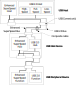
\includegraphics[width=0.6\textwidth]{dual-bus}
	\caption{Dual bus architecture, (Figure 3-1 from \cite{usb3})}
	\label{fig:dual-bus}
\end{figure}

There are three cases of a pair of devices connecting. The simplest one is
a USB 3 device/hub connecting to a USB 3 hub. Both devices handshake and use
only the Enhanced Superspeed Bus. When a USB 2 device is plugged into USB~3
hub, the hub will recognize it, and use only the USB 2 bus. The last case, USB
2 device connecting to USB 2 hub, follows the specification of USB 2.

The key idea is that every USB 3 device is essentially two devices with a shared
port -- an Enhanced Superspeed device and a USB 2 device, of which only one is
active at the same time. The specification doesn't require the device to have
the same function in both USB 2 and USB 3 modes. For example, the USB~2
function may be used to only describe that the device can only operate in USB 3 mode.

Hubs are a notable exception from the single-mode rule as they are actually
two independent hubs in one box. The inner USB 2 hub connects as an USB
2 device and the USB 3 hub connects as a USB 3 device. When a downstream
device is connected physically it is decided to which inner hub it will be
connected based on the device actual speed.

You can see that USB 3 sort of breaks the rule of backwards compatibility. The
protocol is not backwards compatible on its own, but the specification forces
all USB 3-compliant devices to be USB 2-compliant as well. The majority of
compatibility breaks are on the hardware level though, the protocols are very
similar from the perspective of drivers.

\subsubsection{Differences from USB 2}

USB 3 introduces several new features used to speed up the communication and
offer more bandwidth. Most of these features are hidden to the device drivers.
They will be described in this section.

One of the new features USB 3 introduces is called bursting. An endpoint that
supports bursting states its maximum data burst size in its SuperSpeed Endpoint
Companion descriptor. When a transfer is initiated the sender may send multiple
packets in a row before it has to wait for an explicit handshake. This
eliminates the wait time and improves the communication efficiency.

Unlike USB 2 and previous versions where the bus was half-duplex, the bus in USB
3 is full duplex. This means that a device using USB 3 may use both IN and OUT
transactions concurrently.

The devices on USB 2 bus communicate using broadcast. For OUT transactions,
every hub broadcasts the packet to all enabled downstream ports and only the
targeted device should accept the packet. In USB 3, the communication is
routed directly to the receiver. This introduces the need for route strings,
which describe the ports of the hubs on the way to the device.

In USB 2, the controller is required to poll the device to offer it an
opportunity to finish an interrupt transfer. Using the full-duplex links, USB~3
introduces asynchronous notifications to reduce the overhead of polling.

At last but not least, USB 3 introduces more complex power management
features. For example, an USB 3 device may initiate link power state change at
the device while in USB 2, this could be only initiated by the host.
